\chapter{Evolution of the STXS framework}\label{app:merging_schemes}
This Appendix demonstrates the evolution of the STXS framework by providing a schematic of each STXS stage. The stages are defined to accommodate increasing statistics, in the sense that with more p-p collision data, we become sensitive to increasingly granular regions of the Higgs boson production phase space. Therefore, subsequent stages are defined with more kinematic bins. The stage 0, stage 1.0 and stage 1.1 schemes are relevant for the EFT interpretation in Chapter~\ref{chap:eft}, which combines cross sections measurements from multiple decay channels at these stages. The \Hgg analysis in Chapters~\ref{chap:hgg_overview}--\ref{chap:hgg_results} is based on the stage 1.2 binning scheme. 
\section{Stage 0}
\begin{figure}[htb!]
  \centering
  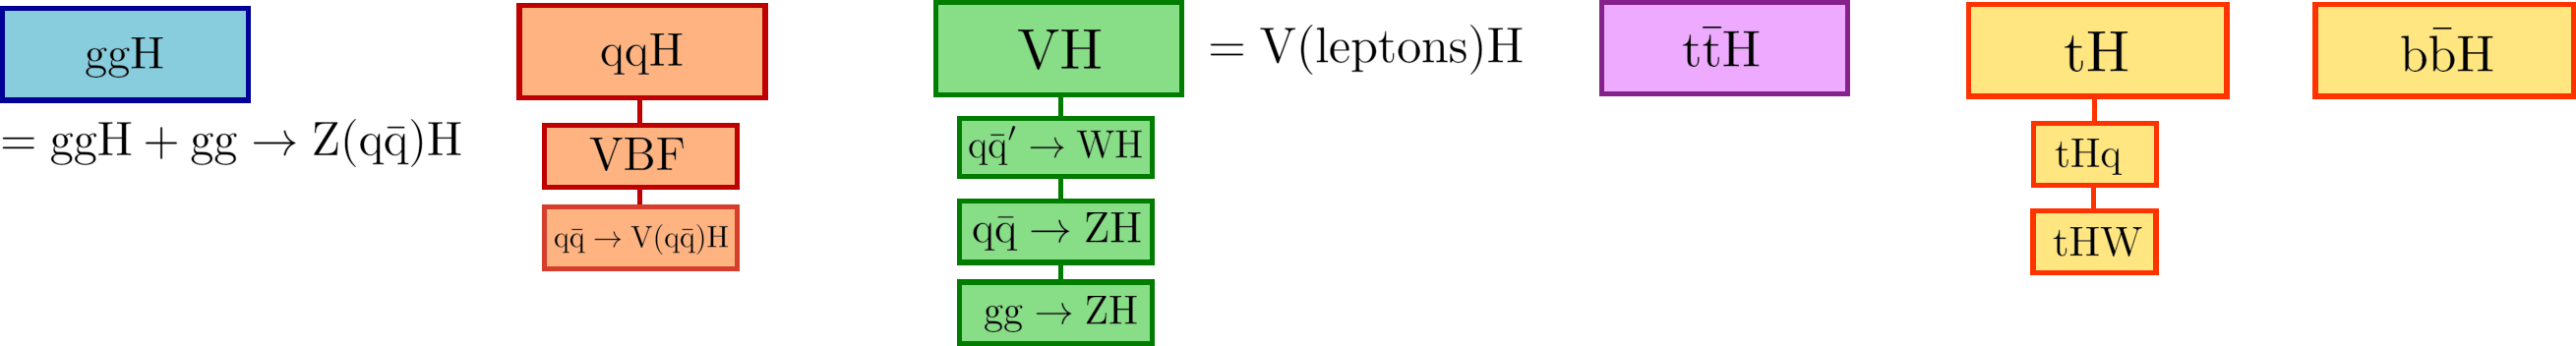
\includegraphics[width=.9\linewidth]{Figures/app_merging_schemes/stage0.pdf}
  \caption[Schematic of the STXS stage 0 binning scheme]
  {
    Schematic showing the STXS stage 0 binning definition. The bins correspond to the different Higgs boson production modes at the LHC.
  }
  \label{fig:stxs_schematic_stage0}
\end{figure}
% \newpage
% \vspace{-.5cm}
\newpage
\FloatBarrier
\section{Stage 1.0}
\begin{figure}[htb!]
  \centering
  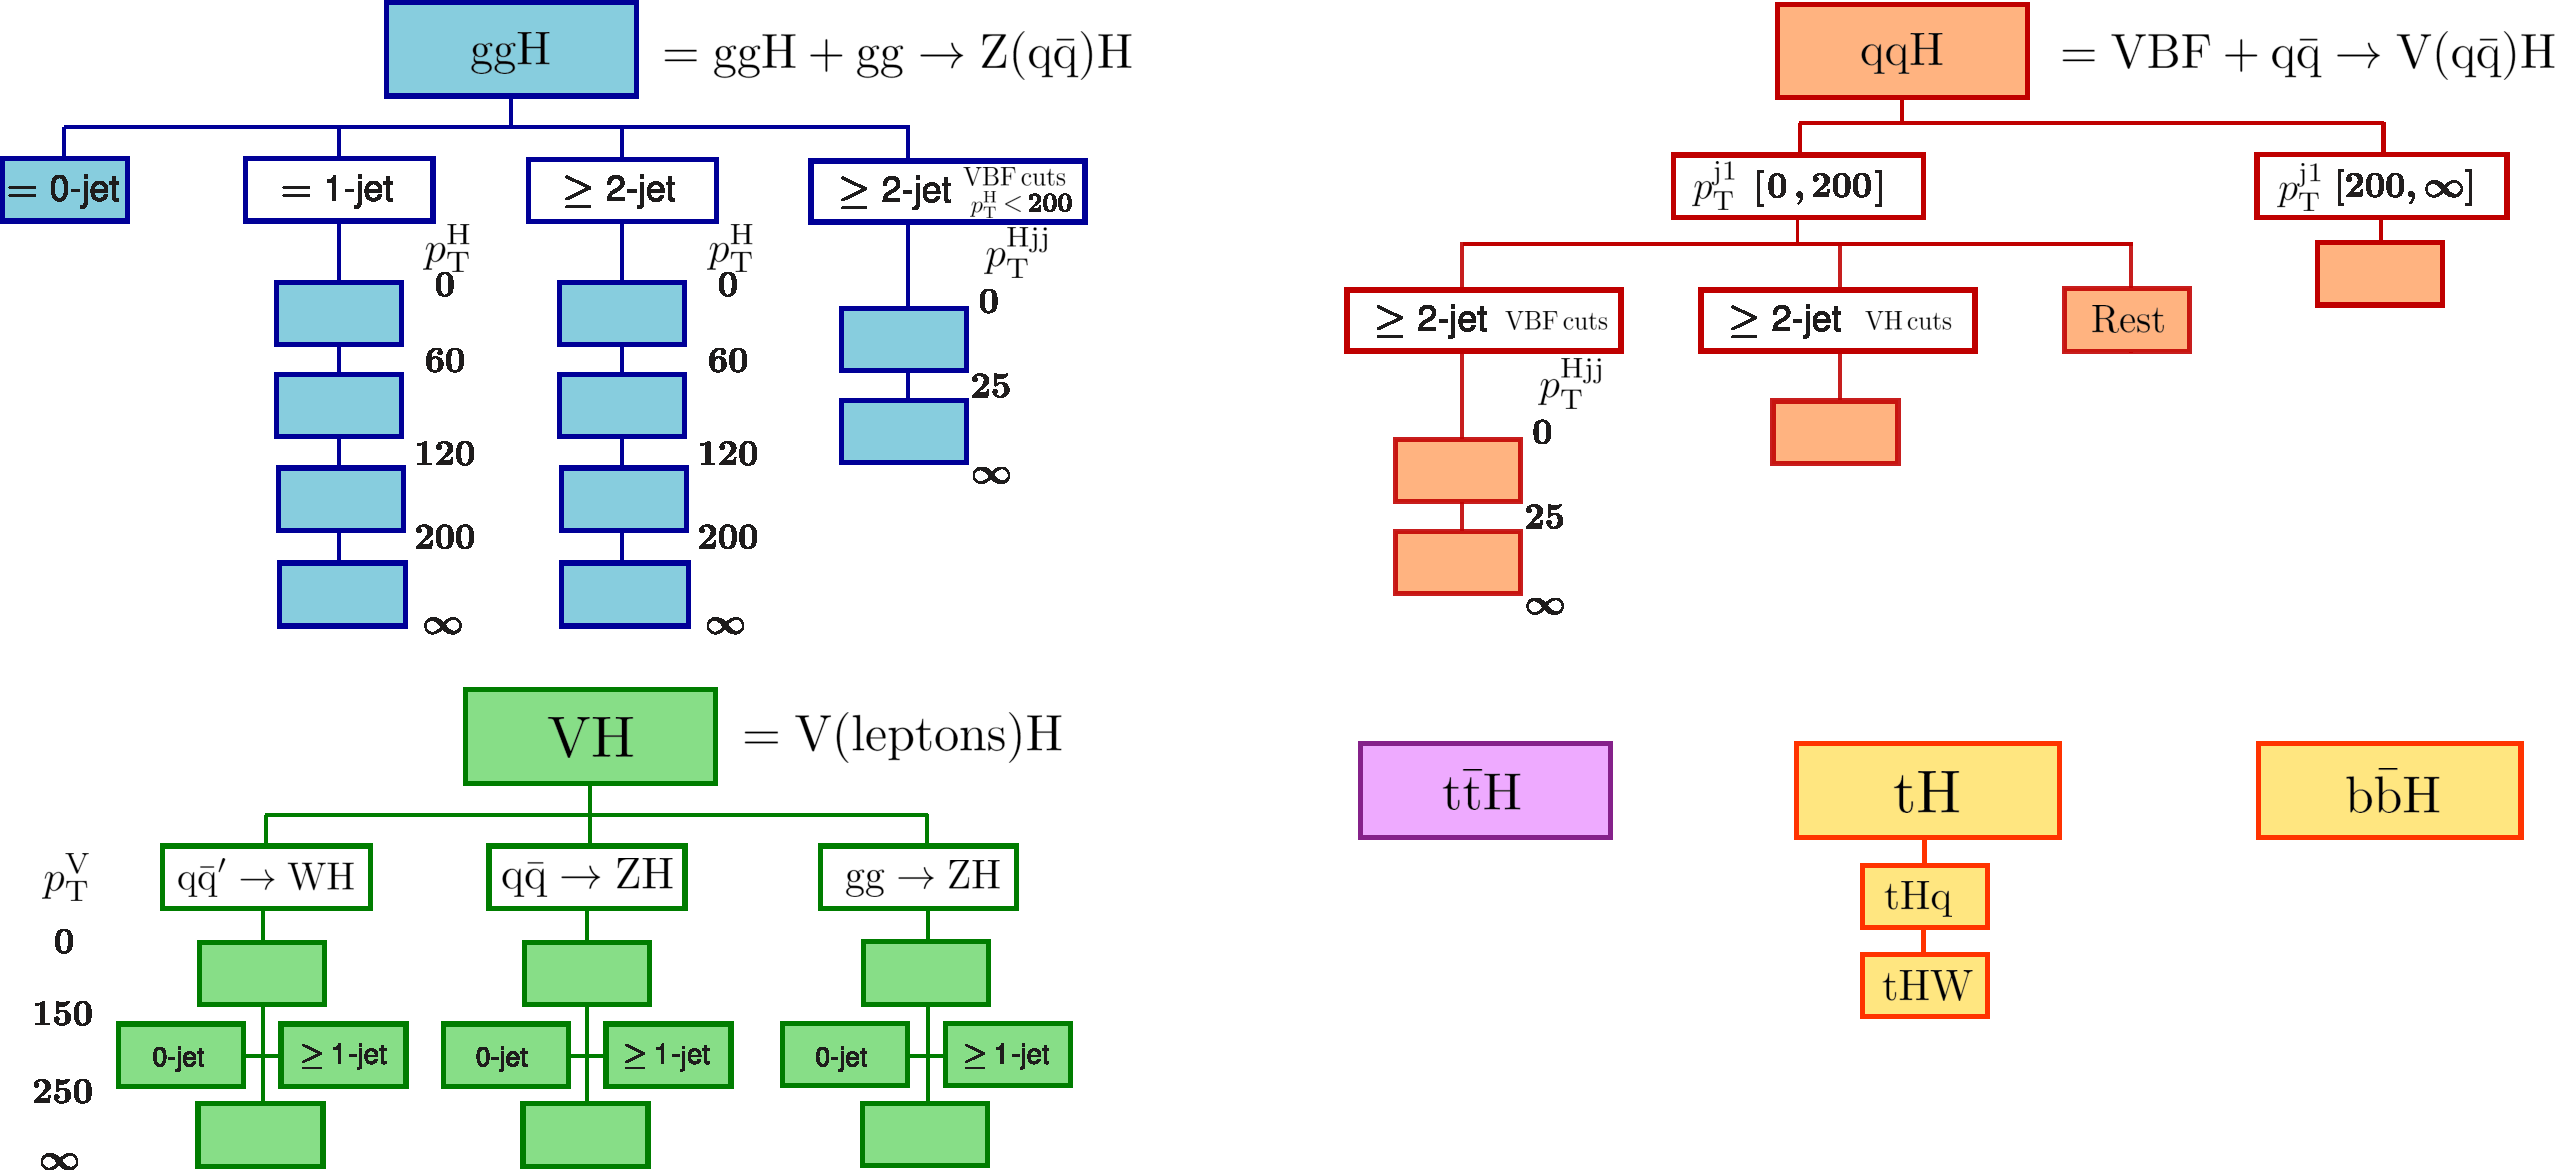
\includegraphics[width=.9\linewidth]{Figures/app_merging_schemes/stage1p0.pdf}
  \caption[Schematic of the STXS stage 1.0 binning scheme]
  {
    Schematic showing the STXS stage 1.0 binning definition. Here, the ggH, qqH and VH leptonic production modes are split by the event kinematics for the first time. The ``VBF cuts" require the dijet invariant mass, $m_{jj}>400$~GeV, and the difference in pseudorapidity between the jets, $\Delta\eta_{jj}>2.8$. The ``VH cuts" require $60<m_{jj}<120$~GeV.
  }
  \label{fig:stxs_schematic_stage1p0}
\end{figure}
% \vspace{-.5cm}
\FloatBarrier
\section{Stage 1.1}
\begin{figure}[htb!]
  \centering
  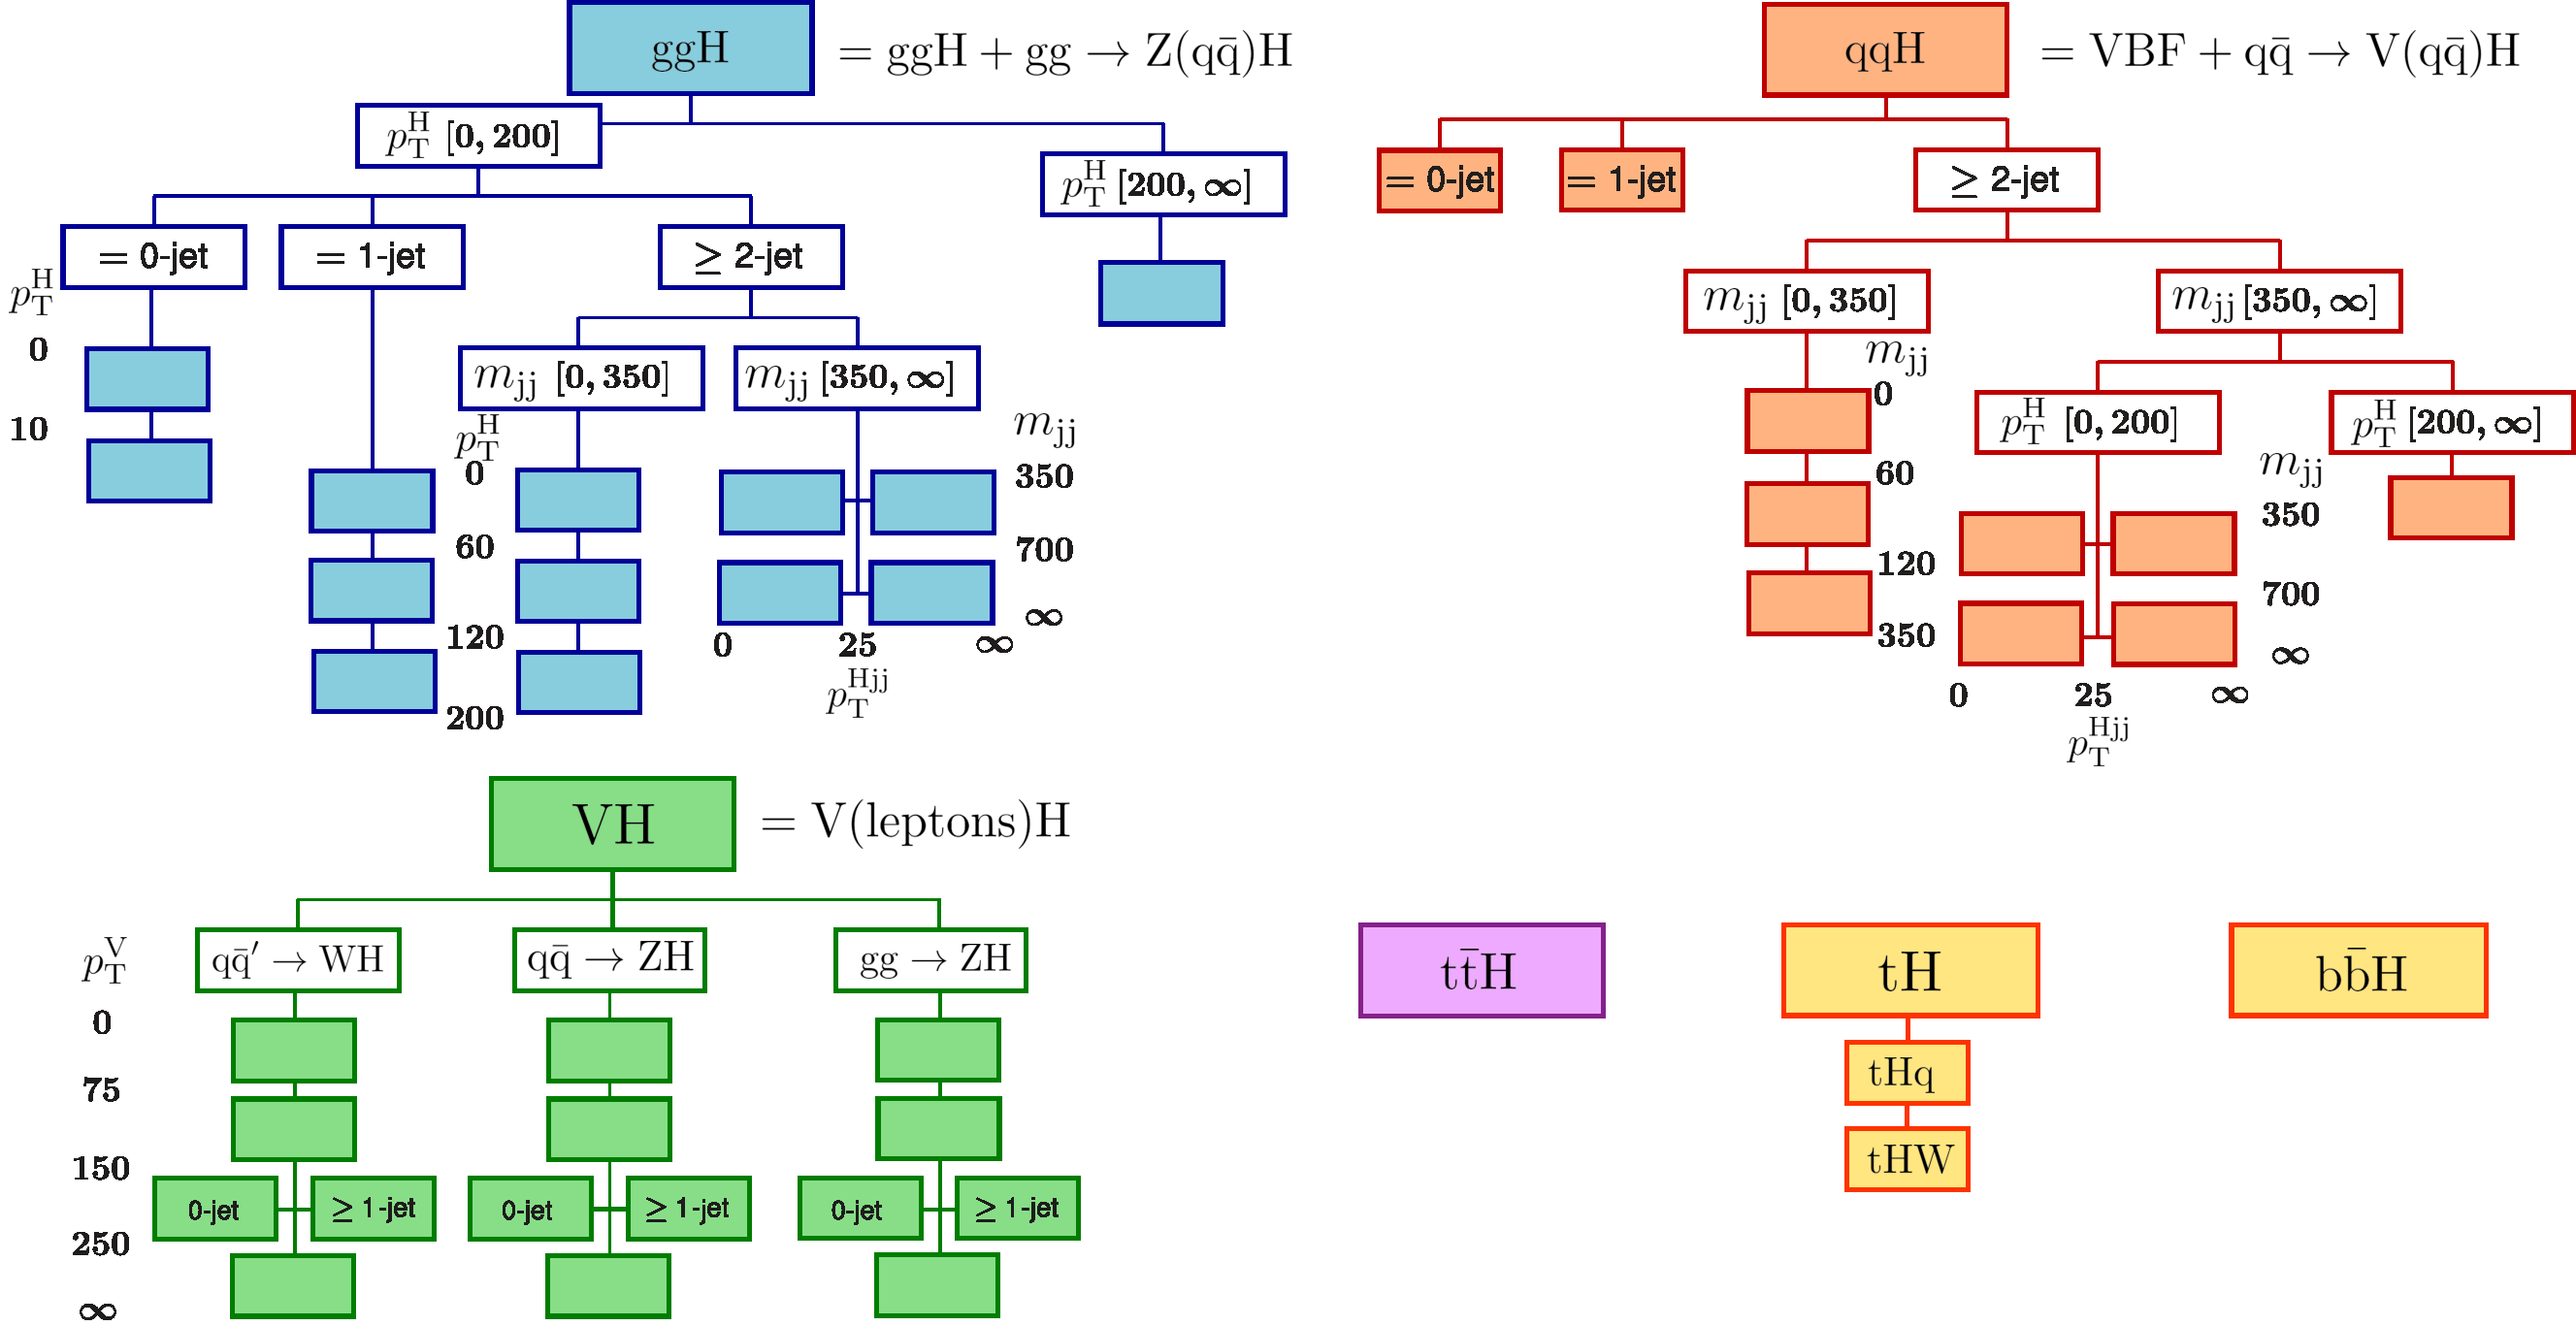
\includegraphics[width=.95\linewidth]{Figures/app_merging_schemes/stage1p1.pdf}
  \caption[Schematic of the STXS stage 1.1 binning scheme]
  {
    Schematic showing the STXS stage 1.1 binning definition. The ggH and qqH binnings are significantly revised with respect to the stage 1.0 scheme. Additionally, the VH leptonic bins include an extra splitting at $p_T^V=75$~GeV.
  }
  \label{fig:stxs_schematic_stage1p1}
\end{figure}
\vspace{-.5cm}
\FloatBarrier
\section{Stage 1.2}
\begin{figure}[htb!]
  \centering
  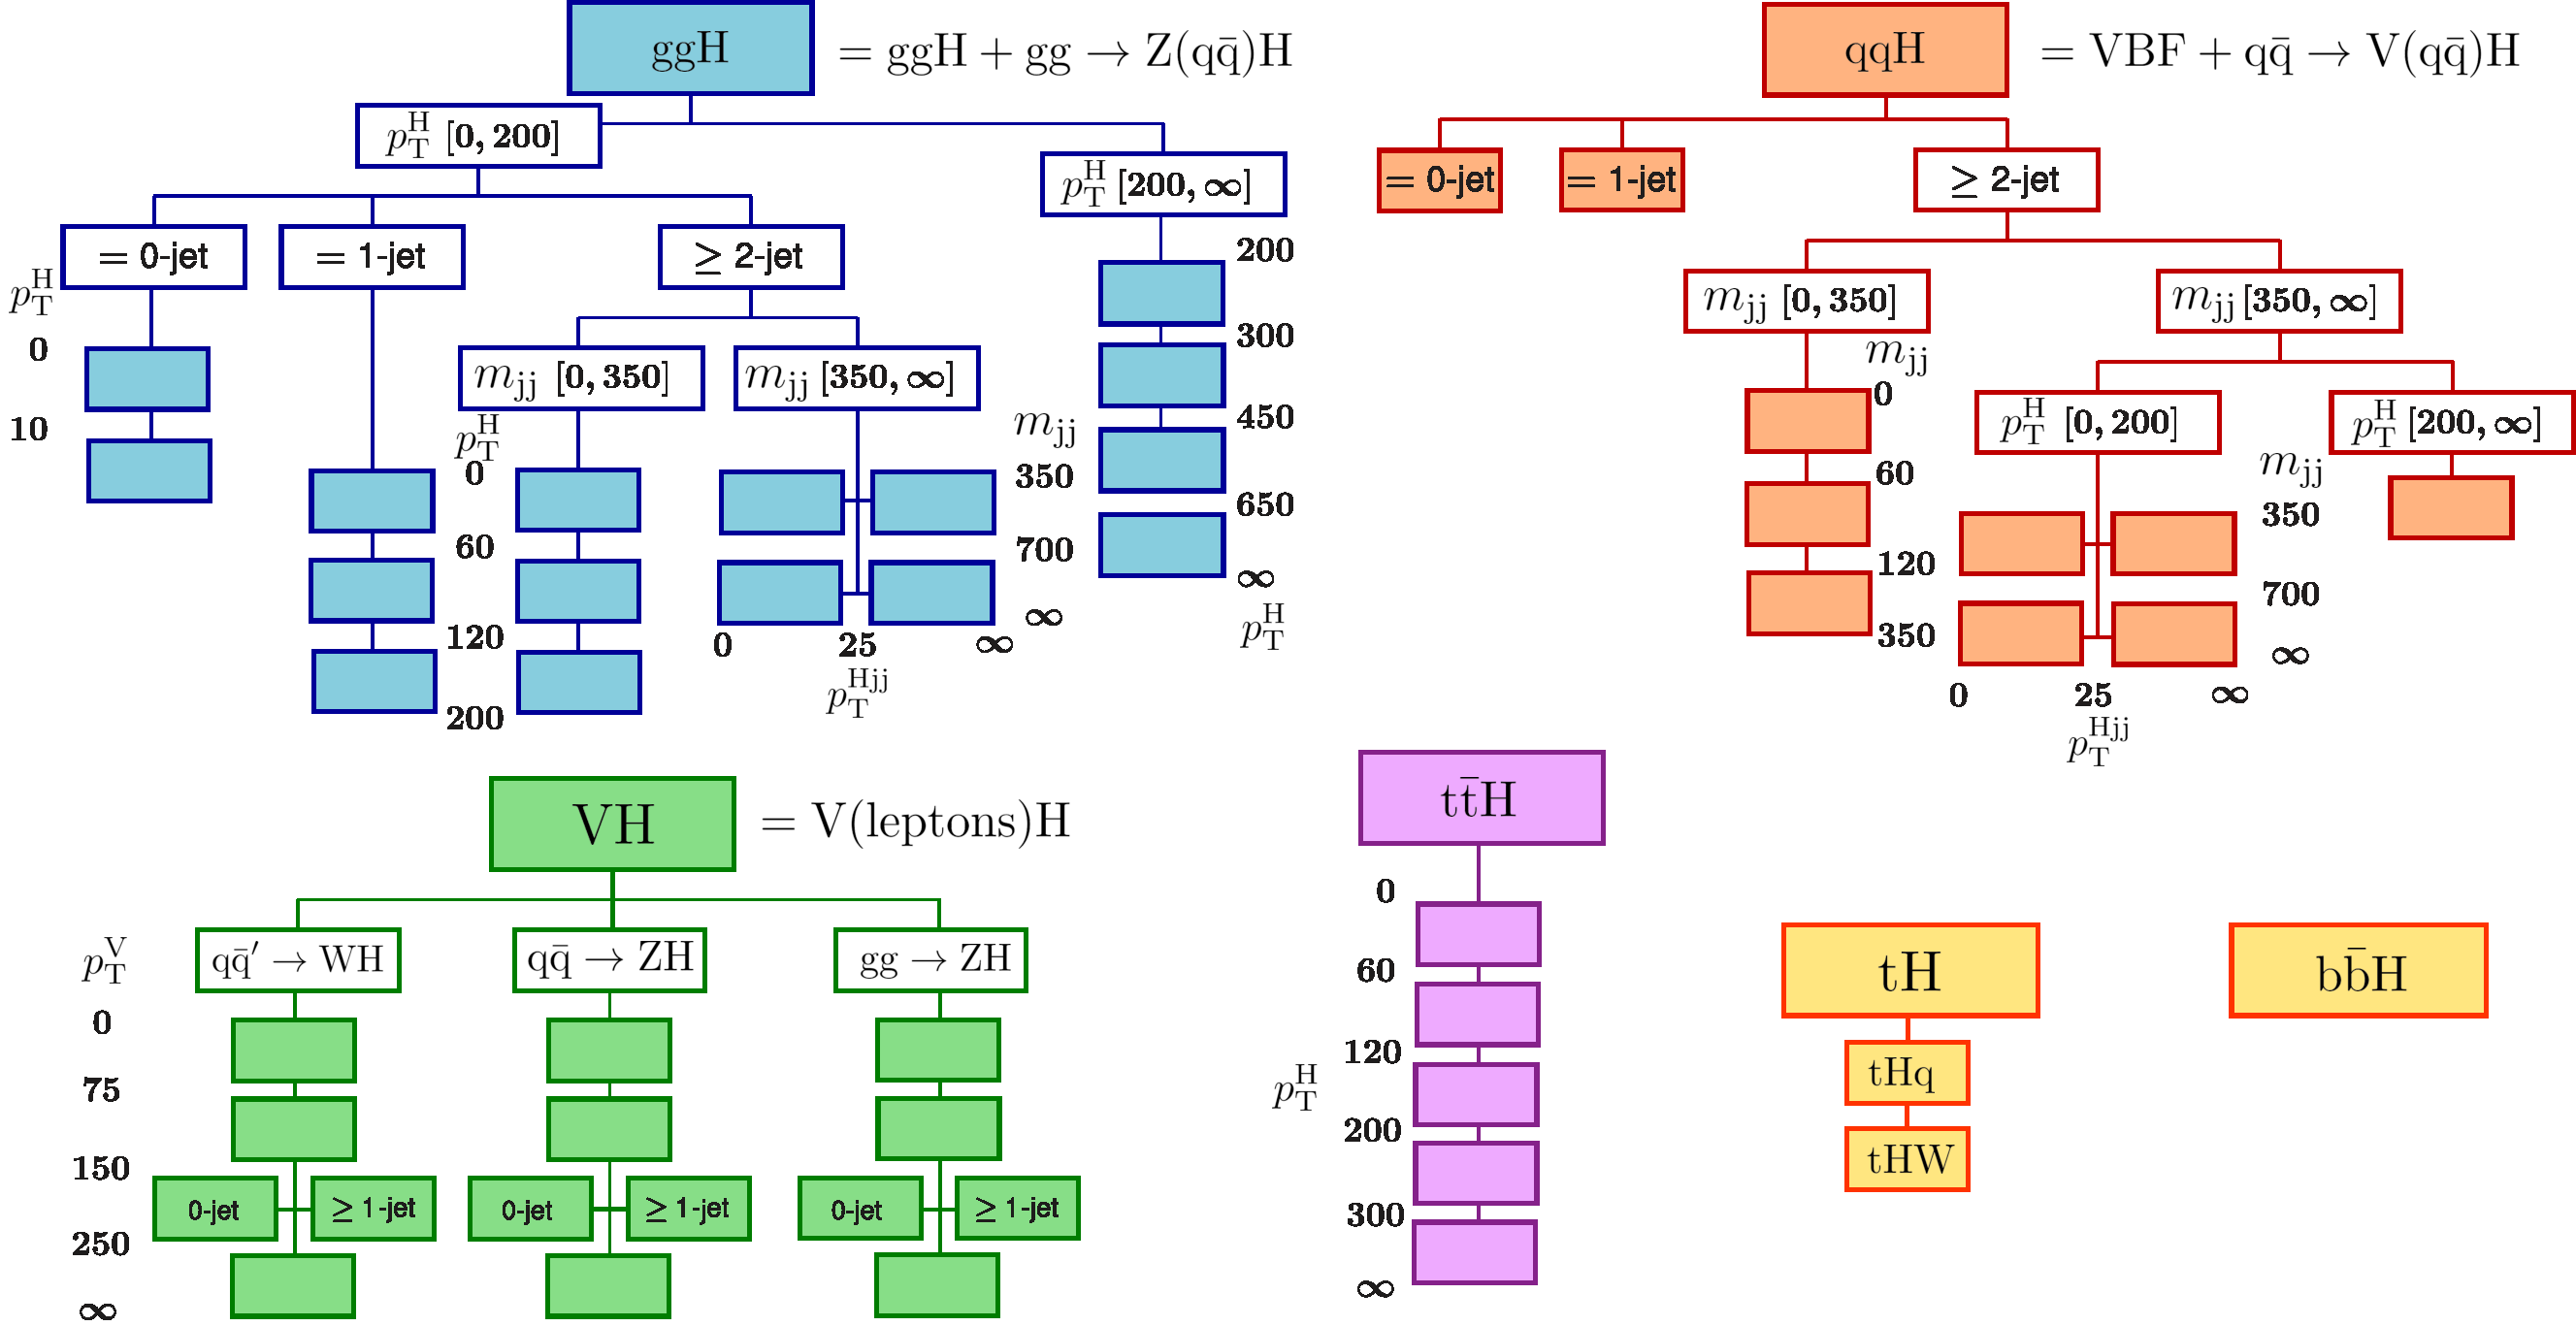
\includegraphics[width=.95\linewidth]{Figures/app_merging_schemes/stage1p2.pdf}
  \caption[Schematic of the STXS stage 1.2 binning scheme]
  {
    Schematic showing the STXS stage 1.2 binning definition. With respect to the stage 1.1 scheme, the ggH BSM region with $p_T^H>200$~GeV is split into four bins according to $p_T^H$ boundaries. Also, the ttH production mode is split here for the first time, into five separate $p_T^H$ bins.
  }
  \label{fig:stxs_schematic_stage1p2}
\end{figure}
